
		\paragraph{QuizziPedia::Front-End::Directives::TrainingSetUpDirective}
		
		\label{QuizziPedia::Front-End::Directives::TrainingSetUpDirective}
		
		\begin{figure}[ht]
			\centering
			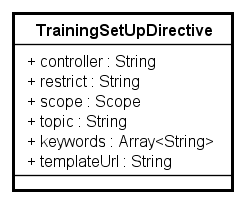
\includegraphics[scale=0.80,keepaspectratio]{UML/Classi/Front-End/QuizziPedia_Front-end_Templates_TrainingSetUpTemplate.png}
			\caption{QuizziPedia::Front-End::Directives::TrainingSetUpDirective}
		\end{figure} \FloatBarrier
		
		\begin{itemize}
			\item \textbf{Descrizione}: rappresenta il componente grafico che permette all'utente di selezionare l'argomento e le parole chiave per iniziare un allenamento con queste caratteristiche. Viene visualizzato dinamicamente all'interno della view TrainingView mediante il controller TrainingController;
			\item \textbf{Utilizzo}: viene utilizzato per consentire all'utente di selezionare l'argomento e le parole chiave di un allenamento;
			\item \textbf{Relazioni con altre classi}: 
			\begin{itemize}
				\item \textbf{IN \texttt{TrainingModelView}}: classe di tipo \textit{modelview\ped{G}} la cui istanziazione è contenuta all'interno della variabile di ambiente \textit{\$scope} di \textit{Angular.js\ped{G}}. All'interno di essa sono presenti le variabili e i metodi necessari per il \textit{Two-Way Data-Binding\ped{G}} tra la view \texttt{TrainingView} e il controller \texttt{TrainingController};
				\item \textbf{OUT \texttt{TrainingView}}: view principale della modalità allenamento. Conterrà i vari templates di ogni domanda dell'allenamento;  
				\item \textbf{IN \texttt{LangModel}}: rappresenta il modello delle informazioni per la giusta traduzione dell'applicazione.
			\end{itemize}
			\item \textbf{Attributi}:
			\begin{itemize}
				\item \textit{+ topic: String} \\ Valore ottenuto come risultato dal ciclo effettuato sull'array degli argomenti;
				\item \textit{+ keywords: Array[String]} \\ Valore ottenuto come risultato dal ciclo effettuato sull'array delle keywords;
				\item \texttt{+ controller: String} \\ Stringa contenente il nome del controller della direttiva;
				\item \texttt{+ restrict: String} \\ Stringa che permette di definire le modalità di inserimento della direttiva all'interno della pagina;
				\item \texttt{+ scope: Scope} \\ Oggetto \texttt{\$scope} interno della direttiva, contiene le funzionalità per gestire i dati presenti all'interno;
				\item \texttt{+ templateUrl: String} \\ Stringa contenente il percorso del file \textit{HTML\ped{G}} che contiene la direttive.
			\end{itemize}
		\end{itemize}
		